\part{ОПТИМИЗАЦИЯ}
    Метод Гаусса-Зейделя ($GZ_1$) сводит задачу поиска наименьшего значения функции нескольких переменных к многократному решению одномерных задач оптимизации, по сути - это постепенное, в многократном цикле, сдвигание к результату по координатным ортам.
    \section*{Алгоритм метода оптимизации $GZ_1$}
        \begin{center}
            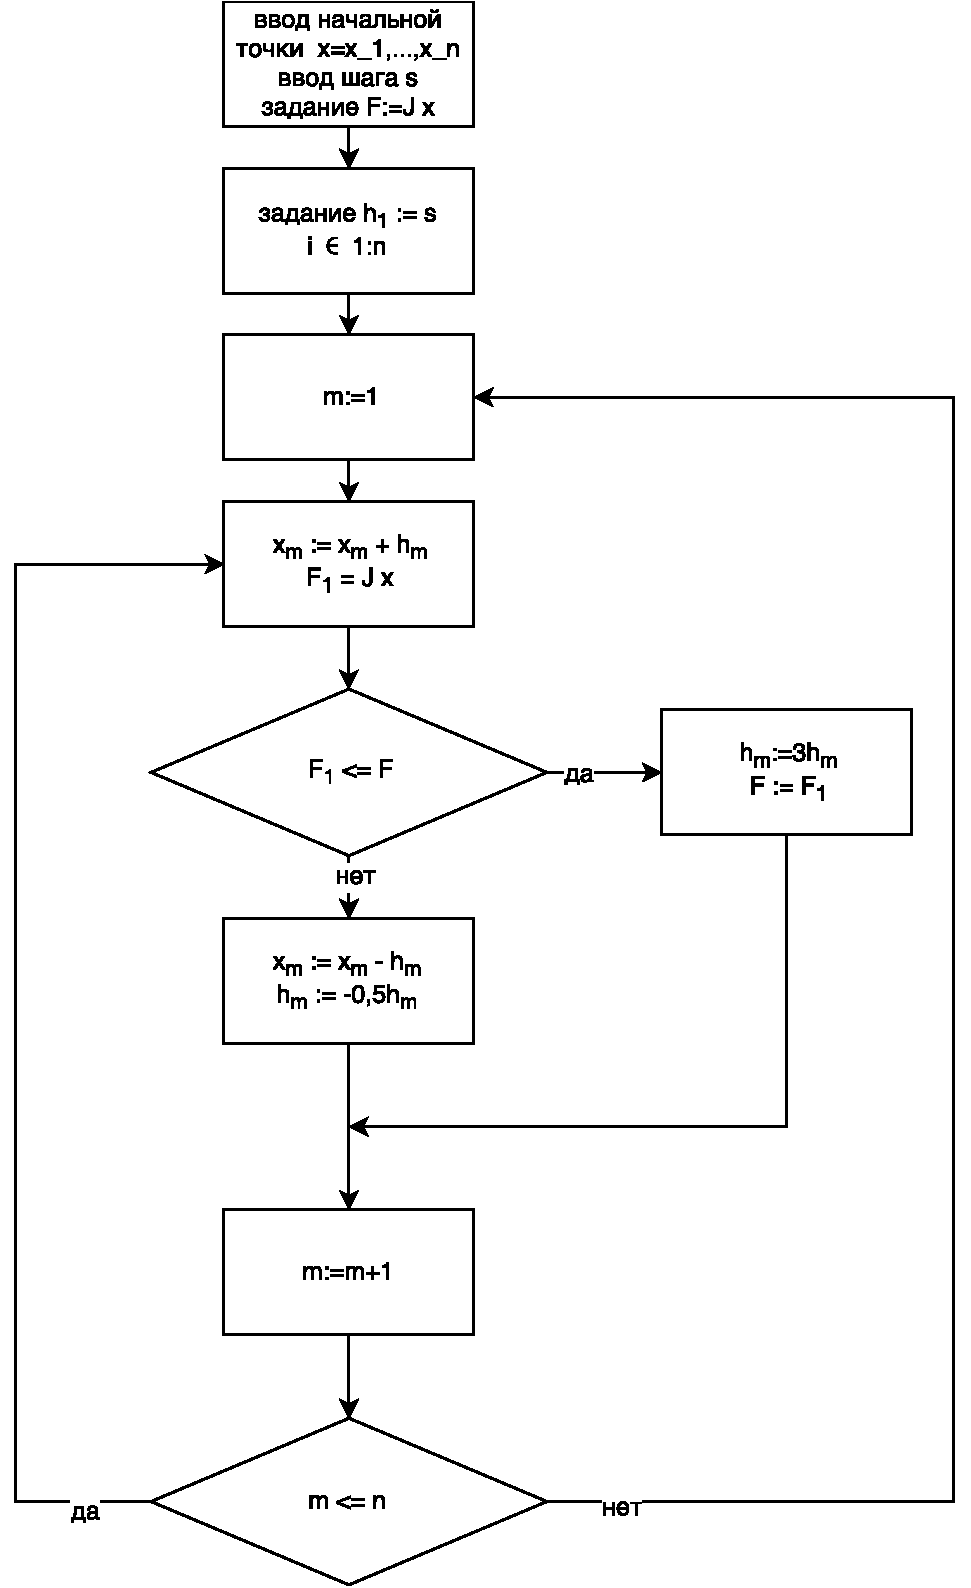
\includegraphics[scale=0.7]{img/gz1-alg}
        \end{center}
        Выход из алгоритма осуществляется по достижении заданного числа вычислений $J$ или при достижении необходимой сходимости.

    \section*{Проверка работоспособности}
        \subsection*{Функция эллипса $r^2 = x^2 + y^2$}
            \begin{tikzpicture}
                \begin{axis}[
                        width=16cm,
                        height=10cm,
                        xlabel=x,
                        ylabel=y,
                        minor tick num = 1,
                        grid = both
                    ]
                    \addplot table [col sep=comma, x index=1, y index=2] {data/precomputed/ellipse.csv};
                \end{axis}
            \end{tikzpicture}

            Точка минимума $(0;0)$

        \subsection*{Функция Розенброка $z = (1 - x)^2 + 100 \times (y - x^2)^2$}
            \begin{tikzpicture}
                \begin{axis}[
                        width=16cm,
                        height=10cm,
                        xlabel=x,
                        ylabel=y,
                        minor tick num = 1,
                        grid = both
                    ]
                    \addplot table [col sep=comma, x index=1, y index=2] {data/precomputed/rosenbrock.csv};
                \end{axis}
            \end{tikzpicture}

            Точка минимума $(1;1)$

        Из представленных выше графиков можно сделать вывод о том, что метод оптимизации реализован верно.
